%
% File acl2014.tex
%
% Contact: giovanni.colavizza@epfl.ch
%%
%% Based on the style files for ACL-2013, which were, in turn,
%% Based on the style files for ACL-2012, which were, in turn,
%% based on the style files for ACL-2011, which were, in turn,
%% based on the style files for ACL-2010, which were, in turn,
%% based on the style files for ACL-IJCNLP-2009, which were, in turn,
%% based on the style files for EACL-2009 and IJCNLP-2008...

%% Based on the style files for EACL 2006 by
%%e.agirre@ehu.es or Sergi.Balari@uab.es
%% and that of ACL 08 by Joakim Nivre and Noah Smith

\documentclass[11pt]{article}
\usepackage{acl2014}
\usepackage{times}
\usepackage{url}
\usepackage{latexsym}

\usepackage[margin=1in]{geometry}
\usepackage{amsmath,amsthm,amssymb, graphicx, multicol, array}

%\setlength\titlebox{5cm}

% You can expand the titlebox if you need extra space
% to show all the authors. Please do not make the titlebox
% smaller than 5cm (the original size); we will check this
% in the camera-ready version and ask you to change it back.


\title{Official works with private tools}

\author{Rehan Mulakhel \\
  {\tt \{rehan.mulakhel\}} \\\And
  Brice Repond \\
  {\tt \{brice.repond\}} \\\And
  Kenneth Nguyen \\
{\tt \{kenneth.nguyen\}\{@epfl.ch\}} \\}

\date{}

\begin{document}
\maketitle
\begin{abstract}
Quickly identifying topics from a relatively large amount of textual messages could not be done efficiently a few decades ago. In this paper, we will compare results obtained from a naive algorithm based on key words system coupled with external knowledge against the well known linear regression, on Hillary Clinton emails. 
\end{abstract}

\section{Introduction}

The Hillary Clinton email controversy arising from the use of private email server for official communications during her tenure as Secretary of State hit the headline of the media in 2015. However the content of the emails was not covered properly and reading relevant information related to it remains a difficult task. The goal of this project is to get some insight from the sensitive and sometimes confidential information publicly available online. We will use the content of the emails and the network of the connection to draw conclusions.

\section{Datasets description}

Kaggle provides the same data in two different formats: four csv files VS one sqlite file. We only consider the former because the operations we will perform require the built in functions of pandas. The raw data with dimensions have the following shapes:

\begin{itemize}
    \item \texttt{emails.csv} (7945, 22)
    \item \texttt{persons.csv} (513, 2)
    \item \texttt{aliases.csv} (850, 3)
    \item \texttt{email\_receiver.csv} (9306, 3)
\end{itemize}

Theses tables form an entity relationship diagram. One would expect the emails to be linked somehow to the persons and the persons to be linked to the aliases. However, the raw data is based on the fields of the emails rather than the structure of a well designed database. Indeed, emails fields use (textual!) aliases to join the tables. Therefore, it is not possible to get the value of the persons directly from the emails.

The reasons for this inconvenient choice is likely due to the fact that the data were generated before the creation of the structure storing it. The one who gathered the data stopped the process at an early stage, leaving us to fend ourselves. Actually, the few extracted values such as the content are not useful because of the poor quality.

Data cleaning is the step which will take the most time. Since we are interested in Hilary's network and the topics covered in the messages, we keep the source of the emails, the destination and the carbon copy (cc) if any, the date and the content.

\section{Exploration and data cleaning}

In general, it is not possible to organize the work in a cascade fashion when working with potentially dirty data. Going back and forth cannot be avoided and is required to understand the data. Understanding the data is necessary to improve the cleaning actions or to recover from missing or unusable values. There are easy mistakes or bad design choice we can observe by simply over reading columns. There are hidden mistakes which cannot be spot without carefully reading and \emph{expecting} some values.

\subsection{Aliases and Persons}

The relation between persons and aliases tables would normally be one-to-many. However, there are some closed aliases pointing to different persons. For instance, `monica.hanle' alias is not pointing towards the same identifier as `Monica Hanley' as one could reasonably expect. Solving this issue can be done through many algorithms like clustering by the Hammer distance and/or by the longest shared string. This would solve most of the wrong links but some exceptions would be uncaught. Since the number of rows is small, clustering the aliases manually is likely to take less time than implementing the algorithms with the exceptions. Eventually, we reduce the size of the persons table by around a third which is not negligible.

\subsection{Emails}

The subject of an email cannot always be deduced from its content because all messages have an implicit context. The same sentence does not necessarily have the same meaning all the time. It depends on too many parameters like the person who wrote it and the moment when it was written and the social conventions at the time when it was written...

\subsubsection{Distribution over time}

\begin{figure}[h]
	\centering
	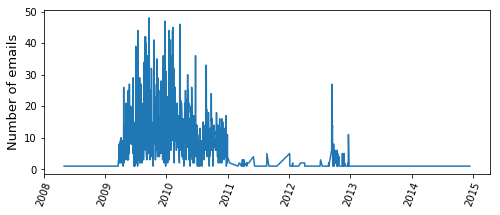
\includegraphics[width=\linewidth]{images/emails_distribution.png}
	\caption{Time distribution of all the emails}
	\label{fig:emails_time_distribution}
\end{figure}

The Figure \ref{fig:emails_time_distribution} shows three periods we call `contexts' we identify them as:

\begin{itemize}
    \item \texttt{ctx0} from 2009 to 2011
    \item \texttt{ctx1} from 2011 to 2012 June
    \item \texttt{ctx2} from 2012 June to 2013
\end{itemize}

We should keep in mind that some emails may have not been or could have not been disclosed.

It is hard to give an interpretation without introducing external knowledge. We can map the second periods to the Libya intervention in 2011 and the third one to the murder of US ambassador in Libya.

\subsubsection{Sender and Receiver}

The sender column is partially filled with the \texttt{personId} field and 157 \texttt{NaN}. The remaining \texttt{Nan} values by extracting them from the content by the first occurrence of an non-empty line starting by the chars: `From:'. 146 \texttt{NaN} remain in the end.

The receiver column contains a string of an alias. Hence, we would like to use the table \texttt{email\_receivers} which contains the value of the receivers. Unfortunately, the table makes no difference between the main receivers and people to whom the message was copied. Therefore, we fetch the value of \texttt{personId} through the aliases table. At this point, we recover 7671 out of 7690 (because we only consider not-\texttt{NaN} rows). Following the same procedure as for the sender does not help because that is what was done by the one extracted the value for us...

How can we complete the unknown values? Verifying whether or not the first row appearing in the receiver table is the main receiver shows that There are 1244 emails for which we have the destination \emph{and} for which there are at least 2 rows in \texttt{email\_receivers}. Among those 1244, the first row is the destination 795 times. This number is not huge but it is not small either. Assuming this ratio always holds, it is better to adopt this strategy than choosing randomly. In the end we have not recover a significant number of missing values.

\subsubsection{Content}

A typical email is composed of a sender, a receiver, a time stamp and a content. Some emails are made of many replies. Sometimes the replies come from the same person. We decided to keep those emails as single emails. This will not hurt the results too much since the thread of conversations should be related to the same topics in most cases.

In order to extract the content from the \texttt{RawText} field which contains the content in addition to metadata in a single string, we perform two phases of process we call pre and post-process.

During the pre-process, we filter out the rows starting by common words like `From:' or `To:' and others which appear in all the emails we have read. Next, we lower all the chars, remove the emails using a regex before combining the split lines into a single line because most sentences are break. From this point, the pipeline is easy to describe, we keep only letters, we stem words and keep them if their length is bigger than 1 and the word is not in the stop list provided by NLTK, we keep sentences having at least 3 words. We join all the sentences with the pipe char ($|$).

At this stage, printing all words starting by the string `afg' returns: afg, afganistan, afgh, afgha, afghaiistai, afghalistan, afghan, afghani, afghanisan, afghanist, afghanistan, afghansn, afghanstan, afghariistan, afghathtml, afgna. This shows that we are working with misspelled words. Ideally, one would find a way to recover as much as possible from these frequent errors. But we will keep things simple and let it how it is. During the post-process, we remove the frequent words by setting the threshold of the tf-idf at 3.4. We got this value by testing manually and observing the output of the words which would be removed.

\section{Topics detection}

The size of the dataset is too small to get valid results using common machine learning tools. We have $|\{ emails \}| << |\{ words \}|$. On the other hand, there are potentially a huge number of topics appearing in the few emails we have. The conditions are met for an overfit. We will use two different techniques to discover information: one basic and naive way based on key words, and one more complex based on logistic regression, hoping to reach the same conclusions.

\subsection{Key words}

Enriching data is a common task in data science. It could be useful to map an email to one or many places on the Earth. We consider the following: North America, Latino world, Europe, Africa, Middle East, Central Asia, Far East, Russia (including Ukraine). Each of these columns is a boolean and one email can be situated in more than a single place. One naive system can determine the position based on some key words appearing in the content of the emails. The results of this solution need to be taken with cautious because it contains a lot of false positive when frequent words are used as key words, and a lot of false negative when important words are missing. For our case, we can expect `Obama' to appear frequently even when the content is not related to the United States.

\subsubsection{Emails distribution per region}

If we consider all the dataset and not the feature `North America', emails are dominated by the Middle East and Europe, followed by Central Asia, Far East then Africa. Latino world and Russia do not seem to be concern to much by the emails compared to the others. We will neglect that and consider only the distribution within what we call \texttt{ctx}. 

If we take the plot in Figure \ref{fig:emails_map_distribution_ctx0}, then it not a surprise to observe the same distribution as the one we have for the whole dataset. It is because the majority of emails were sent during this moment.

\begin{figure}[h]
	\centering
	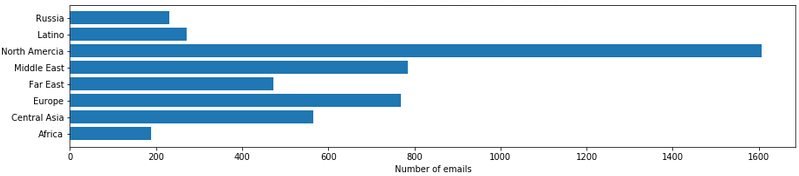
\includegraphics[width=\linewidth]{images/emails_map_ctx0.png}
	\caption{Region distribution in \texttt{ctx0}}
	\label{fig:emails_map_distribution_ctx0}
\end{figure}

For the \texttt{ctx1} in Figure \ref{fig:emails_map_distribution_ctx1}, the place dominating is the Africa, followed by Europe and Middle East.

\begin{figure}[h]
	\centering
	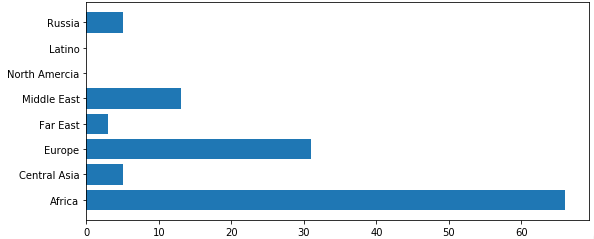
\includegraphics[width=\linewidth]{images/emails_map_ctx1.png}
	\caption{Region distribution in \texttt{ctx1}}
	\label{fig:emails_map_distribution_ctx1}
\end{figure}

For the last context in Figure \ref{fig:emails_map_distribution_ctx2}, we see that Africa is again dominating but Middle East beats Europe.

\begin{figure}[h]
	\centering
	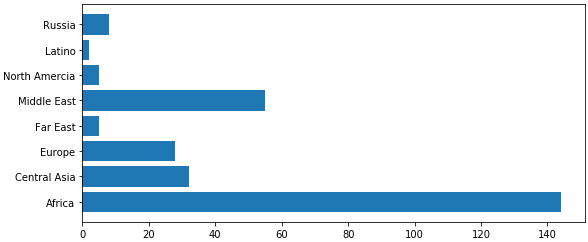
\includegraphics[width=\linewidth]{images/emails_map_ctx2.png}
	\caption{Region distribution in \texttt{ctx2}}
	\label{fig:emails_map_distribution_ctx2}
\end{figure}

The plots based on key words lead us to the hypothesis we have drawn based on the distribution of the emails date.

\subsection{Machine learning}

The input of our machine learning algorithm are not emails but sentences. The target value will be the three contexts we observe in Fig TODO. The goal is to learn the topics covered in each context.

The regularization parameter is taken at the moment when we see the (cross validation) score decreasing.

The result we get are the following

\begin{description}
    \item[Context 0] Afghanistan, China, Iraq
    \item[Context 1] Libya (Qaddafi, NATO, fight, rebel), Egypt (Morsi)
    \item[Context 2] US Ambassador killed in Benghazi, Morocco, Tunisia, Islam and Muslim (probably because of the movie Innocence of Muslims), Romney
\end{description}

The above result are computed based on sentences

We can visually see how close are the emails using dendograms. We do not check on the context 0 because it contains too many elements and the plot would be impossible to interpret.

\begin{figure}[h]
	\centering
	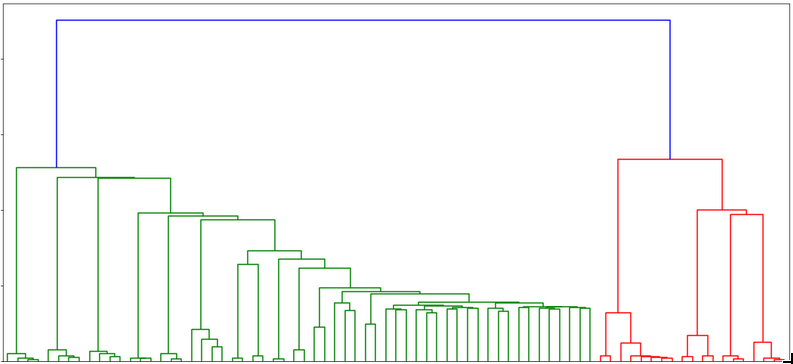
\includegraphics[width=\linewidth]{images/dendogram_ctx1.png}
	\caption{Proximity hierarchy in \texttt{ctx1}.}
	\label{fig:dendogram_ctx1}
\end{figure}

The Figure~\ref{fig:dendogram_ctx1} shows two classes. One of them is likely to be related to North Africa which includes Libya (NATO, fly zone, ...). We can suppose the other class is related to Mohamed Morsi. We can also suppose Egypt and Libya are in the same cluster and the other one contains topics unrelated to this part of the world and unrelated to each other too.

\begin{figure}[h]
	\centering
	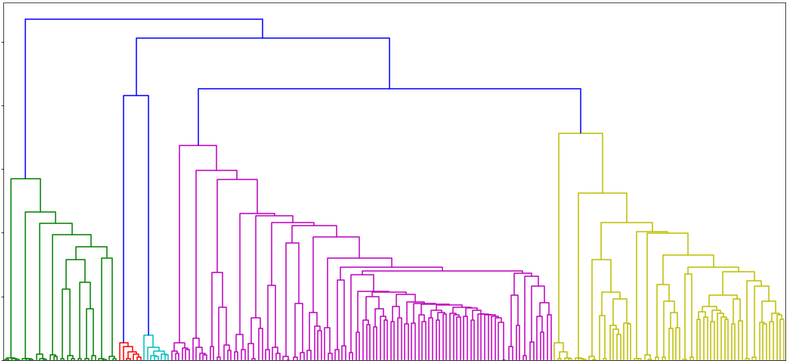
\includegraphics[width=\linewidth]{images/dendogram_ctx2.png}
	\caption{Proximity hierarchy in \texttt{ctx2}.}
	\label{fig:dendogram_ctx2}
\end{figure}

The Figure \ref{fig:dendogram_ctx2} shows three topics dominating. We guess there is one cluster containing emails related to the murder of the US ambassador. Another cluster probably contains events related directly or indirectly to the movie `Innocence of Muslims'.

\section{Visualization tools}

\subsection{Wordcloud and N-grams}
What are the most used words in each region ? In this section, we use two different visualisation tools to detect these words by region. Since we have eight plots, we focus only on one region and we choose Africa and especially with the Libyan war.

\begin{figure}[h]
	\centering
	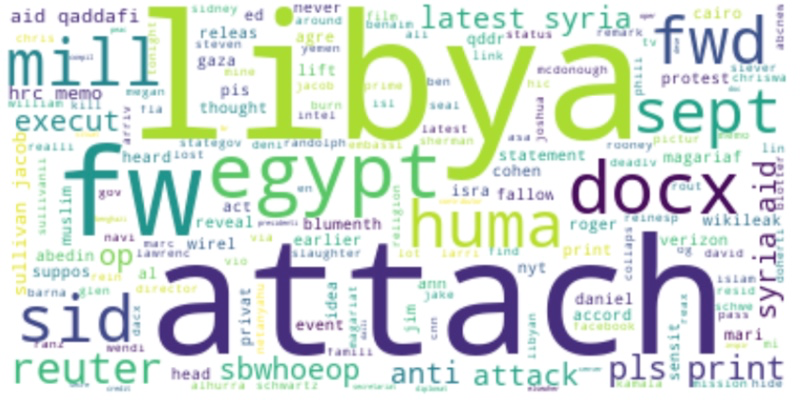
\includegraphics[width=\linewidth]{images/wordcloud_africa.png}
	\caption{wordcloud for Africa.}
	\label{fig:wordcloudaf}
\end{figure}

The Figure \ref{fig:wordcloudaf} shows the most used words in the emails exchanged in Africa, we observe that the most used word is Libya and Egypt, the there is a connection with Figure \ref{fig:dendogram_ctx1} and assume that both words are in the same cluster.
\subsection{Hilary's network}

With whom Hillary Clinton exchanges the most. This is likely the question that interests the most people. We interest in this Section to answer this question. At this aim, we create the Hilary's Network with the people with whom she has the most exchange of emails.

The size of nodes is a relative measure of the total amount of emails that a person has. Similarly, the size of the edges represents the relative number of emails that two persons have each together. The main peers are namely: Huma Abedin, Chery Mills, Jake Sullivan, Lauren Jiloty, Sidney Blumenthal. They are mostly political advisers of Hillary Clinton.

\section{Conclusion}

The naive algorithm based on key words works surprisingly well in this specific case. But it requires a lot of external knowledge and is prone to miss interesting information. On the other hand, the unsupervised algorithm is easier to implement and produces results which are more easy to interpret. In both cases, external knowledge helps to understand the context.

\begin{thebibliography}{}

\bibitem[\protect\citename{Aho and Ullman}1972]{Aho:72}
Alfred~V. Aho and Jeffrey~D. Ullman.
\newblock 1972.
\newblock {\em The Theory of Parsing, Translation and Compiling}, volume~1.
\newblock Prentice-{Hall}, Englewood Cliffs, NJ.

\bibitem[\protect\citename{{American Psychological Association}}1983]{APA:83}
{American Psychological Association}.
\newblock 1983.
\newblock {\em Publications Manual}.
\newblock American Psychological Association, Washington, DC.

\bibitem[\protect\citename{{Association for Computing Machinery}}1983]{ACM:83}
{Association for Computing Machinery}.
\newblock 1983.
\newblock {\em Computing Reviews}, 24(11):503--512.

\bibitem[\protect\citename{Chandra \bgroup et al.\egroup }1981]{Chandra:81}
Ashok~K. Chandra, Dexter~C. Kozen, and Larry~J. Stockmeyer.
\newblock 1981.
\newblock Alternation.
\newblock {\em Journal of the Association for Computing Machinery},
  28(1):114--133.

\bibitem[\protect\citename{Gusfield}1997]{Gusfield:97}
Dan Gusfield.
\newblock 1997.
\newblock {\em Algorithms on Strings, Trees and Sequences}.
\newblock Cambridge University Press, Cambridge, UK.

\end{thebibliography}

\end{document}
